% *- coding: UTF-8 -*-
% !TEX builder = Texlive
% !TEX prggram = xelatex

%文档设置及格式

%文档设置及格式
\documentclass[UTF8,a4paper,12pt,titlepage]{ctexart}
% tittlepage制作一个封面
% draft是草稿,有个方框
%\documentclass[UTF8,a4paper,11pt]{book}

%\CTEXsetup[name={第,章}]{section}%每section统一名称

%每章节题目统一格式
\CTEXsetup[format={\zihao{-3}\raggedright\bfseries}]
{section}

\newcommand{\keyword}[1]{\textbf{#1}}


% 纸张格式
\usepackage[paper=a4paper,inner=1.5cm,outer=2cm,top=2cm,
bottom=2.5cm,bindingoffset=0.5cm]{geometry}

\usepackage[onehalfspacing]{setspace} % 1.5倍行距

% 自动链接内容(网页链接)
\usepackage[colorlinks=true,linkcolor=black]{hyperref}



% 设置文件属性内容
\hypersetup{pdfauthor={吴毓明},
            pdftitle={PAM制备投加装置},
            pdfsubject={使用说明},
            pdfkeywords={任何问题,联系61508712@qq.com}}

% 定义页眉页脚
% 定义页眉页脚
\usepackage{fancyhdr}
\fancyhf{}
\pagestyle{fancy}
% 公共
\rhead{\zihao{6}一体化全自动加药装置/化工泵\\
       Manage Pump as Diamond} % 页眉右

% 利亨昌
% \lhead{
\includegraphics{LHC-head.png}}% 页眉左
% \lhead{
\includegraphics[height=0.5cm]{LHC.jpg}} % 页眉左
% \chead{\zihao{4}广州市利亨昌贸易有限公司}
% \chead{\zihao{5}广州市利亨昌贸易有限公司}
% \lfoot{\zihao{6}广州市荔湾区东联路2号工业园\\
%                电话:020-8430 1397 传真:020-84301170 \\ 
%                电邮:gzlhcmy@163.com 网址:www.lhcmy.com}
% \cfoot{\thepage} % 页脚右
% \cfoot{\zihao{5}\thepage} % 页脚中
% \rfoot{\zihao{6}美国帕斯菲达PULSAFEEDER 产品库存商\\Paddle-flow流量监控及加药装置} % 页脚右
% \rfoot{\zihao{6}美国帕斯菲达PULSAFEEDER 产品库存商\\Paddle-flow流量监控及加药装置} % 页脚右
% \rfoot{\thepage} % 页脚右

% paddle-flow
%\rhead{\includegraphics{paddle-flow.png}}

% 厦门飞华
\lfoot{厦门飞华环保有限公司}
\rfoot{\thepage} % 页脚右



\renewcommand{\headrulewidth}{0.4pt} % 页眉分隔线
\renewcommand{\footrulewidth}{0.4pt} % 页脚分隔线

% 表格格式定义
% 表格 定义表头字体
\newcommand{\head}[1]{\textnormal{\textbf{#1}}}

% 表格 特殊命令,见后文 array
% 在竖向多种对齐方式
\usepackage{array}
\setlength{\extrarowheight}{4pt} % 增加列距
\usepackage{booktabs} % 用于美化表格的线
\usepackage{multirow} % 合并行
\newcommand{\normal}[1]{\multicolumn{1}{l}{#1}}


% 图片
% 图片处理
\usepackage{graphicx}
\usepackage{wrapfig} % 文字环绕图片

% 流程图
% 导入tikz绘图包
\usepackage{tikz}
% 导入基本图形
\usetikzlibrary{shapes,arrows}
%说明文字
\tikzstyle{text_box} = [
   rectangle,
   rounded corners,
   minimum width=1.5cm,
   minimum height=0.5cm,
   text centered, 
   ]
%箭头
\tikzstyle{arrow} = [thick,->,>=stealth]



% 特殊符号(例如千分号等)
\usepackage{textcomp}

% 开始正文
\begin{document}

% 制作封面
\title{
   \zihao{1} PAM自动制备投加装置\\[2.5mm]
   \zihao{1} 使用说明及注意事项\\
   {\noindent}\rule{16cm}{1pt}\\[3mm]
   % \zihao{2} 广州市利亨昌贸易有限公司\\
   \zihao{2} 厦门创洁数智环保水处理科技有限公司\\
   % \zihao{4} 吴毓明\\
   %\zihao{4} Wym\\
   %\zihao{4} 2022年12月27日
   \begin{figure}[h]
      \centering
      \includegraphics[height=10cm]{p9.PNG}
   \end{figure}
}

\maketitle % 封面



\tableofcontents % 目录

\newpage % 换页

%\part{系统组成}
%ctex的\chapter{sdsg}是不能用的
\section{系统组成及功能说明}

   PAM制备投加装置的主要组成部分,如下图\ref{fig:p1}或图\ref{fig:p2}所示。
   \subsection{系统构成图}

   % 系统构成图
   % 图片模板
      \begin{figure}[h]
         \centering

         \begin{tikzpicture}
            %定义图像
            \node at (0,0) {\includegraphics[height=14cm]{p11.PNG}};

            %说明
            \node at (-6,5) (1) [text_box] {进水流量探头};
            \draw [arrow] (1) -- (-2.5,1.1);
            \node at (4,-6) (2) [text_box] {进水口};
            \draw [arrow] (2) -- (1.6,-4.4);
            \node at (2,-7) (3) [text_box] {排液口};
            \draw [arrow] (3) -- (0.4,-5);
            \node at (6,-5) (4) [text_box] {加药口};
            \draw [arrow] (4) -- (5.3,-3.2);
            \node at (-2,-6) (5) [text_box] {放空阀};
            \draw [arrow] (5) -- (-0.3,-4.6);
            \node at (-4,-6) (6) [text_box] {放空阀};
            \draw [arrow] (6) -- (-1.5,-3.8);
            \node at (-6,-4) (7) [text_box] {放空阀};
            \draw [arrow] (7) -- (-3,-3);
            \node at (-6,-5) (8) [text_box] {进水阀};
            \draw [arrow] (8) -- (-1,-3);
            \node at (-7,-3) (9) [text_box] {Y型过滤器};
            \draw [arrow] (9) -- (-2.3,-2.3);
            \node at (0,7) (10) [text_box] {搅拌机};
            \draw [arrow] (10) -- (-0,3);
            \node at (5,4) (14) [text_box] {搅拌机};
            \draw [arrow] (14) -- (2.5,2.5);
            \node at (6,3) (15) [text_box] {超声波液位计};
            \draw [arrow] (15) -- (1.5,1.5);
            \node at (3,5) (17) [text_box] {螺旋进料器};
            \draw [arrow] (17) -- (0,1);
            \node at (-7,1) (18) [text_box] {进水电动阀};
            \draw [arrow] (18) -- (-1.4,0.5);
            \node at (-7,0) (19) [text_box] {进水压力表};
            \draw [arrow] (19) -- (-1,0.4);
            \node at (-5,6) (20) [text_box] {料斗};
            \draw [arrow] (20) -- (-2.5,3.5);
            \node at (-7,-1) (21) [text_box] {进水压力变送器};
            \draw [arrow] (21) -- (-0.5,0.3);

			% 辅助线
             %\def \xLimit {8};
             %\def \yLimit {8};
             %
			% 辅助线
            \draw (-\xLimit,-\yLimit) [help lines] grid (\xLimit,\yLimit);
            \foreach \x in {-\xLimit, ...,\xLimit}{
               \node [red] at (\x, \yLimit) {\x};
               \node [red] at (\x, -\yLimit) {\x};
               \node [red] at (\x, 0) {\x};
            }
            \foreach \y in {-\yLimit, ...,\yLimit}
                  \node [red] at (-\xLimit, \y) {\y};
            \foreach \y in {-\yLimit, ...,\yLimit}
                  \node [red] at (\xLimit, \y) {\y};
            \foreach \y in {-\yLimit, ...,\yLimit}
                  \node [red] at (0, \y) {\y};


         \end{tikzpicture}
         \caption{PAM制备系统组成}\label{fig:p1}
      \end{figure}



\newpage % 换页

   % 系统构成图
   
      \begin{figure}[h]
         \centering

         \begin{tikzpicture}
            %图片
            \node at (0,0) {\includegraphics[height=12cm]{p1.PNG}};

            %说明
            \node at (5,6) (1) [text_box] {电控柜};
            \draw [arrow] (1) -- (3,4);
            \node at (6,3) (2) [text_box] {稀释水流量探头};
            \draw [arrow] (2) -- (2,2.2);
            \node at (0,6) (3) [text_box] {背压阀};
            \draw [arrow] (3) -- (-0.4,0.2);
            \node at (-2,5) (4) [text_box] {安全阀/泄压阀};
            \draw [arrow] (4) -- (-0.7,-0.1);
            \node at (6,-3) (5) [text_box] {计量泵};
            \draw [arrow] (5) -- (2,-0.5);
            \node at (3,-5) (6) [text_box] {计量泵};
            \draw [arrow] (6) -- (0,-1.5);
            \node at (-4,4) (7) [text_box] {阻尼器};
            \draw [arrow] (7) -- (-1.7,0.5);
            \node at (2,7) (8) [text_box] {隔膜压力表};
            \draw [arrow] (8) -- (0.9,1.6);
            \node at (6,1) (9) [text_box] {隔膜压力表};
            \draw [arrow] (9) -- (2.2,1.2);
            \node at (-5,-5) (10) [text_box] {Y型过滤器};
            \draw [arrow] (10) -- (-1.3,-3.9);

			% 辅助线
            %\def \xLimit {8};
            %\def \yLimit {8};
            %
			% 辅助线
            \draw (-\xLimit,-\yLimit) [help lines] grid (\xLimit,\yLimit);
            \foreach \x in {-\xLimit, ...,\xLimit}{
               \node [red] at (\x, \yLimit) {\x};
               \node [red] at (\x, -\yLimit) {\x};
               \node [red] at (\x, 0) {\x};
            }
            \foreach \y in {-\yLimit, ...,\yLimit}
                  \node [red] at (-\xLimit, \y) {\y};
            \foreach \y in {-\yLimit, ...,\yLimit}
                  \node [red] at (\xLimit, \y) {\y};
            \foreach \y in {-\yLimit, ...,\yLimit}
                  \node [red] at (0, \y) {\y};


         \end{tikzpicture}
         \caption{PAM投加系统组成}\label{fig:p2}
      \end{figure}


   \subsection{系统功能说明}
      PAM自动制备投加装置主要分为自动制备系统和 投加装置两部分组成。
      \par操作人员只需要设定好控制参数,系统将自动运行。
      \subsubsection{自动制备系统功能}
         自动制备系统将PAM固体粉料制备成溶液。
         \par主要设定参数:
         \begin{itemize}
            \item 溶液制备量。制备系统设计制备能力为1000L/h。
            \item 溶液浓度。常用浓度为1\textperthousand $\sim$ 4\textperthousand。
            \item 开机液位。储液池液位低于开机液位时,制备系统自动开机。
               客户可自行设置开机液位,
               出厂默认设置值为0.5米。
            \item 停机液位。储液池液位高于停机液位时,制备系统自动停机。
               客户可自行设置停机液位,
               出厂默认设置值为0.8米,
               设置值不可高于0.9米。
            \item 搅拌机间歇运行参数。
            搅拌机每运行若干分钟,
            则停止若干分钟,
            时长可设置。
            出厂默认设置值为每运行120分钟,
            则暂停5分钟。
            当系统处于溶液制备状态,
            螺旋进料器启动,
            进水电动阀打开时,
            搅拌机将持续运行,
            不会暂停。
            \item 进水低水压。
            进水压力低于此值制备系统自动停机,出厂设置值为2bar。
         \end{itemize}
         \par制备系统自动运行时,
         控制系统根据进水流量探头反馈,
         通过进水电动阀,
         将进水流量控制在上述设定的溶液制备量上。
         \par同时,控制系统根据上述设定参数,
         按以下公式\ref{powder-in}计算出螺旋进料器进料量(kg/h),
         控制进料器电机变频器,
         使进料量达到设定值。
         \begin{equation}
            \label{powder-in}
            \mbox{进料量}(kg/h) = \mbox{溶液制备量}(L/h)  \times \mbox{溶液浓度} (\%)
         \end{equation}
         \par制备系统料斗带有高、低料位报警探头,
         料斗料位过低进会自动停止溶液制备过程并发出报警。
         此时应使用真空上料机吸取PAM原料,
         物料足够时制备系统会恢复自动运行。

      \subsubsection{投加系统功能}
         投加系统
         按设定参数
         向投加点投加PAM溶液。
         \par主要设定及显示参数:
         \begin{itemize}
            \item 各投加泵变频电机频率。调节范围0 $\sim$ 50Hz。
            \item 各投加泵投加流量,单位L/h。
            \item 储液池低液位报警设置,单位m。
            低于此液位PAM溶液不足,
            自动停泵。
               出厂默认设置值为0.2米。
            \item 储液池高液位报警设置,单位m。
               出厂默认设置值为0.9米。
         \end{itemize}

        % 自动稀释功能
        
\subsubsection{自动稀释功能}
    自动稀释功能:
    根据PAM投加计量泵的投加流量,
    按照设定稀释比例,
    向投加管内注入稀释水,
    将投加PAM稀释至设定浓度。
    \par主要设定及显示参数:
    \begin{itemize}
        \item 手动、自动切换。手动控制时,可手动调整电动阀门开度,一般用检查检修电动阀门。
            自动控制时,由PLC自动控制阀门开度,调节稀释水加入流量。
        \item 稀释水电动阀开度 手动调节。调节范围0 $\sim$ 100\%。
        \item 稀释水电动阀当前开度显示。
        \item 稀释比例设定。
            以药剂为1,稀释水为倍数。
            例如:稀释倍数设为3,当前药剂投加流量为10L/h,则稀释水流量将控制为30L/h。
        \item 稀释水当前流量显示。
     \end{itemize}



\newpage % 换页

\section{设备启动前准备}\label{sec:sg1}
   \subsection{紧固件检查}
      系统启动前,要先对所有的紧固件进行检查。
      紧固件包括底座固定螺栓、泵固定螺栓、马达连接螺栓以及所有的法兰连接螺栓等。
      如有松动情况,请将其上紧,如有脱落等情况,请按相应的规格补充相关的螺栓。

   \subsection{管道连接检查}
      检查管道中所有活接接头连接,如有松脱情况需要重新上紧。

   \subsection{检查系统中各阀门状态}
      \subsubsection{各检修阀门应处于关闭状态}\label{sec:sg2}
         检修阀门包括检修排液阀、
         检修旁通阀、放空阀等,
         正常运行时均应处于关闭状态。

         % 各检修阀位置
         % 图片模板
      \begin{figure}[h]
         \centering

         \begin{tikzpicture}
            %定义图像
            \node at (0,0) {\includegraphics[height=13cm]{p11.PNG}};

            %说明
            \def \itemNumber {1};
            \def \centertPoint {-3.9,1.1};
            \node at (-7,3) (\itemNumber) [text_box] {检修旁通阀};
            \draw [arrow] (\itemNumber) -- (\centertPoint);
            \draw (\centertPoint) circle (0.5)[red];
            \def \itemNumber {2};
            \def \centertPoint {-0.3, -4.2};
            \node at (-2,-6) (\itemNumber) [text_box] {放空阀};
            \draw [arrow] (\itemNumber) -- (\centertPoint);
            \draw (\centertPoint) circle (0.5)[red];
            \def \itemNumber {3};
            \def \centertPoint {-1.5, -3.5};
            \node at (-4,-5) (\itemNumber) [text_box] {放空阀};
            \draw [arrow] (\itemNumber) -- (\centertPoint);
            \draw (\centertPoint) circle (0.5)[red];
            \def \itemNumber {4};
            \def \centertPoint {-2.8, -2.8};
            \node at (-6,-4) (\itemNumber) [text_box] {放空阀};
            \draw [arrow] (\itemNumber) -- (\centertPoint);
            \draw (\centertPoint) circle (0.5)[red];
            %\def \itemNumber {5};
            %\def \centertPoint {-3.4,1.4};
            %\node at (-5,5) (\itemNumber) [text_box] {检修截止阀};
            %\draw [arrow] (\itemNumber) -- (\centertPoint);
            %\draw (\centertPoint) circle (0.5)[red];
            %\def \itemNumber {6};
            %\def \centertPoint {-2.5,0};
            %\node at (-7,0) (\itemNumber) [text_box] {检修截止阀};
            %\draw [arrow] (\itemNumber) -- (\centertPoint);
            %\draw (\centertPoint) circle (0.5)[red];

			% 辅助线
             \def \xLimit {8};
             \def \yLimit {8};
             %
			% 辅助线
            \draw (-\xLimit,-\yLimit) [help lines] grid (\xLimit,\yLimit);
            \foreach \x in {-\xLimit, ...,\xLimit}{
               \node [red] at (\x, \yLimit) {\x};
               \node [red] at (\x, -\yLimit) {\x};
               \node [red] at (\x, 0) {\x};
            }
            \foreach \y in {-\yLimit, ...,\yLimit}
                  \node [red] at (-\xLimit, \y) {\y};
            \foreach \y in {-\yLimit, ...,\yLimit}
                  \node [red] at (\xLimit, \y) {\y};
            \foreach \y in {-\yLimit, ...,\yLimit}
                  \node [red] at (0, \y) {\y};


         \end{tikzpicture}
         \caption{各检修阀位置}\label{fig:p3}
      \end{figure}



\newpage

      \par上图\ref{fig:p3}所示为
      检修排液阀、
      检修旁通阀、
      放空阀等阀门所在位置。
      % \par表示这是一段,新开一段才会自动退2个空格
      \par检修排液阀的作用,
      用于在检修时释放系统压力,
      避免管道内化学品喷射出来。
      \par检修旁通阀的作用,
      是电磁流量计、电动阀、压力变送器、压力表等需要检修时,
      关闭其上下游阀门,
      打开检修旁通阀,
      可在手动状态维持系统运行。
      放空阀的作用,
      在于检修制备槽、熟化槽、储药槽时,
      或长期存放装置暂不使用时,
      将槽内积液排空。
      \par正常工作时应将检修排液阀、检修旁通阀关闭。

        \subsubsection{其余阀门均处于开启状态}
            除上述特别说明之外的所有阀门,在正常工作状态下,都应处于开启状态。

\newpage % 换页

   \subsection{制备投加系统上电}
        \subsubsection{电柜操作面板布局}
        电柜操作面板布局如下图\ref*{fig:p5}所示:

        % 电柜操作面板布局图
        
        \begin{figure}[h]
            \centering
            \begin{tikzpicture}
                %图片
                \node at (0,0) {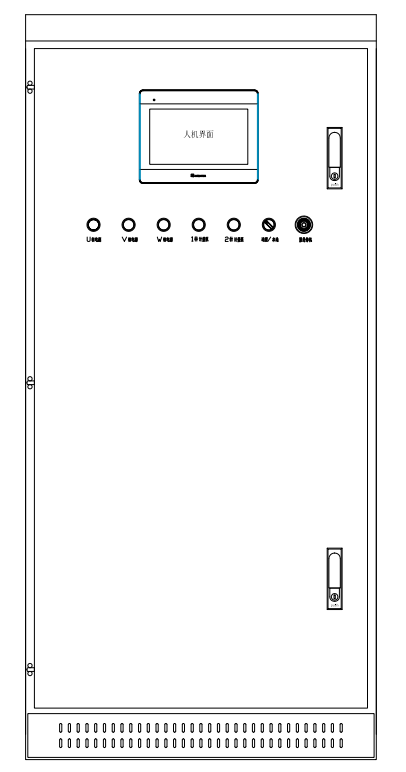
\includegraphics[height=10cm]{g03.PNG}};

                %说明
                \def \itemNumber {1};
                \def \centertPoint {-1.6, 1.8};
                \node at (-2,1.5) (\itemNumber) [text_box] {电柜电源进线指示灯};
                \draw (\centertPoint) rectangle +(1.3,0.5)[red];
                \def \itemNumber {2};
                \def \centertPoint {2,5.5};
                \node at (\centertPoint) (\itemNumber) [text_box] {计量泵运行指示灯};
                \draw [arrow] (\itemNumber) -- (0.3,2);
                \draw (-0.2,1.8) rectangle +(0.7,0.5)[red];
                \def \itemNumber {2};
                \def \centertPoint {0.8, 2.1};
                \node at (1,0) (\itemNumber) [text_box] {远程/在地控制切换};
                \draw [arrow] (\itemNumber) -- (\centertPoint);
                \draw (\centertPoint) circle (0.2)[red];
                \def \itemNumber {3};
                \def \centertPoint {1.3, 2.1};
                \node at (3,1) (\itemNumber) [text_box] {紧急停机按钮};
                \draw [arrow] (\itemNumber) -- (\centertPoint);
                \draw (\centertPoint) circle (0.2)[red];

                % 辅助线
                \def \xLimit {8};
                \def \yLimit {7};
                % 
			% 辅助线
            \draw (-\xLimit,-\yLimit) [help lines] grid (\xLimit,\yLimit);
            \foreach \x in {-\xLimit, ...,\xLimit}{
               \node [red] at (\x, \yLimit) {\x};
               \node [red] at (\x, -\yLimit) {\x};
               \node [red] at (\x, 0) {\x};
            }
            \foreach \y in {-\yLimit, ...,\yLimit}
                  \node [red] at (-\xLimit, \y) {\y};
            \foreach \y in {-\yLimit, ...,\yLimit}
                  \node [red] at (\xLimit, \y) {\y};
            \foreach \y in {-\yLimit, ...,\yLimit}
                  \node [red] at (0, \y) {\y};


            \end{tikzpicture}
            \caption{电柜操作面板布局}\label{fig:p5}
        \end{figure}



        \par电柜电源进线指示灯指示进线电源状态。
        \par计量泵隔膜破裂时,
        计量泵隔膜破裂报警灯会亮,
        计量泵正常时不亮。
        \par远程/在地控制切换旋扭切换控制状态,
        决定由上位机控制还是在地触摸屏控制。
        \par发生突发状况时,
        按下急停按钮,
        所有运行设备均会紧急停机。

      \subsubsection{上电前检查}
         上电之前,
         应先确认电柜电源进线有电,
         且没有缺相。
      \par如上图\ref{fig:p5}所示,
      3个电源指示灯全亮,
      即表示电源进线有电,
      且没有缺相,
      这时可以给电柜上电。

      \newpage % 换页

      \subsubsection{电柜上电}\label{sec:power-on}
        % 电柜内布局
        
         \begin{figure}[h]
            \centering
            \begin{tikzpicture}
               %图片
               \node at (0,0) {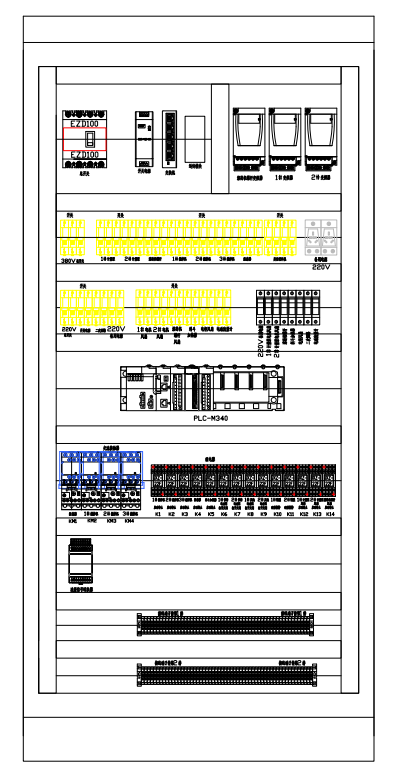
\includegraphics[height=10cm]{g04.PNG}};

               %说明
               \def \itemNumber {1};
               \def \centertPoint {-1.9, 2.7};
               \node at (-3,3) (\itemNumber) [text_box] {电柜总开关};
               \draw (\centertPoint) rectangle +(0.8,0.9)[red];
               \def \itemNumber {2};
               \def \centertPoint {-1.9, 1.5};
               \node at (-3,2) (\itemNumber) [text_box] {其余开关};
               \draw (\centertPoint) rectangle +(3.2,0.7)[red];
               \def \itemNumber {3};
               \def \centertPoint {-1.9, 0.6};
               \node at (-3,1) (\itemNumber) [text_box] {其余开关};
               \draw (\centertPoint) rectangle +(2.4,0.7)[red];

            % 辅助线
               \def \xLimit {8};
               \def \yLimit {7};
            %    
			% 辅助线
            \draw (-\xLimit,-\yLimit) [help lines] grid (\xLimit,\yLimit);
            \foreach \x in {-\xLimit, ...,\xLimit}{
               \node [red] at (\x, \yLimit) {\x};
               \node [red] at (\x, -\yLimit) {\x};
               \node [red] at (\x, 0) {\x};
            }
            \foreach \y in {-\yLimit, ...,\yLimit}
                  \node [red] at (-\xLimit, \y) {\y};
            \foreach \y in {-\yLimit, ...,\yLimit}
                  \node [red] at (\xLimit, \y) {\y};
            \foreach \y in {-\yLimit, ...,\yLimit}
                  \node [red] at (0, \y) {\y};


            \end{tikzpicture}
            \caption{电柜内布局}\label{fig:p6}
         \end{figure}



      \par电柜内布局如上图\ref{fig:p6}所示。
      \par依次打开
      电柜总开关、380V总开关、220V总开关、开关电源开关、
      二次回路开关,
      以及
      1号计量泵、
      2号计量泵、
      溶药机螺杆、
      1号搅拌机、
      2号搅拌机、
      3号搅拌机、
      真空上料机等380V用电设备开关,
      和1号计量泵电机独立冷却风扇、
      2号计量泵电机独立冷却风扇、
      溶药机螺杆独立冷却风扇、
      电柜风扇、
      电磁流量计等220V用电设备开关。

      \par其中,振荡器开关不需要打开。
      振荡器 是在原料比较潮湿,
      并且已经有板结的情况下使用,
      正常情况下不需要使用,
      所以正常情况下不用打开。

      \subsubsection{观察加药装置各系统状态}
      观察人机界面、变频器、PLC及流量仪表工作状态是否正常。
      在正常情况下,人机界面、变频器及流量仪表显示器均应该点亮,PLC上应无红灯闪烁。

      \subsubsection{异常情况处理}
      加药系统上电如发现异常情况,请与加药系统售后服务人员联系。
      如需自行处理,请先详细查阅附件技术资料,自行处理若操作不当,有可能导致加药系统损坏。

\newpage % 换页

\section{日常操作}\label{sec:sg3}
   系统主要通过人机界面进行操作。
      人机界面上的操作界面,
      分为设备操作界面、报警及数据纪录界面两类。
      \par设备操作界面有
      成品投加控制界面、
      溶液制备控制界面、
      反冲洗控制界面3个。
      \par运行状态监控界面 有
      报警记录、
      加药流量曲线、
      电机频率曲线、
      加药历史流量纪录、
      电机频率历史纪录、
      运行累积纪录等6个。

   \subsection{成品投加控制}

      \par成品投加控制界面如下图\ref{fig:p7}所示。
      \par成品投加控制界面
      是系统的主界面,
      可以切换到其他控制界面,
      下图\ref{fig:p7}红圈内为切换到其他控制界面的区域。

      % 成品投加控制界面
        

      \begin{figure}[h]
         \centering
            \begin{tikzpicture}
               %图片
               \node at (0,0) {\includegraphics[height=8cm]{p20.PNG}};

               %说明
               \node at (-5,3) (1) [text_box, color=red] {切换到其他控制界面};
               \draw (-6.5,1.8) rectangle +(3.3,1)[red];

                \def \itemNumber {2};
                \node at (-5,1.5) (\itemNumber) [text_box] {液位报警设置};
                \def \centertPoint {-6.3,-0.9};
                \draw (\centertPoint) rectangle +(3.9,2)[red];
                \draw [arrow] (\itemNumber) -- (-4.5,0);

                \node at (5,3) (3) [text_box] {自动稀释设置};
                \draw (2.4,-0.9) rectangle +(3.9,2)[red];
                \draw [arrow] (3) -- (4,0);

                \node at (-5.5,-3.8) (4) [text_box] {1号计量泵控制};
                \node at (5.5,-3.8) (5) [text_box] {2号计量泵控制};

            % 辅助线
               \def \xLimit {8};
               \def \yLimit {5};
                %
			% 辅助线
            \draw (-\xLimit,-\yLimit) [help lines] grid (\xLimit,\yLimit);
            \foreach \x in {-\xLimit, ...,\xLimit}{
               \node [red] at (\x, \yLimit) {\x};
               \node [red] at (\x, -\yLimit) {\x};
               \node [red] at (\x, 0) {\x};
            }
            \foreach \y in {-\yLimit, ...,\yLimit}
                  \node [red] at (-\xLimit, \y) {\y};
            \foreach \y in {-\yLimit, ...,\yLimit}
                  \node [red] at (\xLimit, \y) {\y};
            \foreach \y in {-\yLimit, ...,\yLimit}
                  \node [red] at (0, \y) {\y};


            \end{tikzpicture}
            \caption{成品投加控制界面}\label{fig:p7}
      \end{figure}


      \par同时,成品投加控制界面
      设置PAM投加系统的运行参数。
            储液池液位低于
            “低液位报警设置”
            的设定时,
            会自动停泵。

            \par在上图\ref{fig:p7}界面设置以下参数:
            \begin{enumerate}
                \item   自动稀释参数。
                    \begin{itemize}
                        \item 稀释控制状态。
                            在自动稀释和 手动稀释之间切换。
                        \item 稀释倍数。
                        以药剂为1,稀释水为倍数。
                        例如:稀释倍数设为3,当前药剂投加流量为10L/h,则稀释水流量将控制为30L/h。
                        \item 稀释水电动阀开度显示。
                        \item 手动阀门开度。
                            手动控制时,设置 稀释水电动阀开度。
                    \end{itemize}
                \item 停泵条件。
                    \begin{itemize}
                    \item 储液池低液位。
                    储液池液位过低时,
                    投加系统自动停泵,
                    出厂设置是0.2m。
                    \end{itemize}
                \item 计量泵控制及显示参数
                    \begin{itemize}
                        \item 变频器故障时,
                            故障状态会亮红灯。
                        \item 计量泵运行时,绿色“运行”灯亮,
                            计量泵停止时,红色“停止”灯亮。
                        \item 计量泵运行频率设置,设置范围是0 $\sim$ 50Hz。
                    \end{itemize}
            \end{enumerate}


   \subsection{溶液制备控制}
       溶液制备控制界面可由主界面(即成品投加控制界面,参考第\pageref{fig:p7}页图\ref{fig:p7})进入。

      \subsubsection{制备参数设置}
      制备系统开始运行前,
      要先设置好制备系统运行参数。

      % 溶液制备控制界面
      

      \begin{figure}[h]
         \centering
            \begin{tikzpicture}
               %图片
               \node at (0,0) {\includegraphics[height=8cm]{p21.PNG}};

               %说明

            % 辅助线
               \def \xLimit {8};
               \def \yLimit {4};
               % 
			% 辅助线
            \draw (-\xLimit,-\yLimit) [help lines] grid (\xLimit,\yLimit);
            \foreach \x in {-\xLimit, ...,\xLimit}{
               \node [red] at (\x, \yLimit) {\x};
               \node [red] at (\x, -\yLimit) {\x};
               \node [red] at (\x, 0) {\x};
            }
            \foreach \y in {-\yLimit, ...,\yLimit}
                  \node [red] at (-\xLimit, \y) {\y};
            \foreach \y in {-\yLimit, ...,\yLimit}
                  \node [red] at (\xLimit, \y) {\y};
            \foreach \y in {-\yLimit, ...,\yLimit}
                  \node [red] at (0, \y) {\y};


            \end{tikzpicture}
         \caption{溶液制备控制界面}\label{fig:p8}
      \end{figure}



      \newpage

      \par在上页图\ref{fig:p8}界面操作方法:
      \begin{enumerate}
         \item 控制权限。
            显示当前控制的权限,
            在上位机或是在地,
            通过电柜面板上的调节旋钮改变。
         \item 控制方式。
            设为手动时,
            可单独手动操作溶液制备过程各相关设备,
            一般是独立测试各设备是否正常时使用。
            手动操作模式时不会有相应联锁,
            例如就算料位低也可以启动进料螺杆,
            应谨慎使用手动控制方式。
            设为自动时,
            系统会根据制备系数设置,
            自动控制溶液制备过程。
         \item 搅拌机控制及设置。
            \begin{itemize}
               \item 启动/停止搅拌机。
                  在手动控制状态,
                  通过启动/停止按钮启停各搅拌机。
                  在自动控制状态,
                  系统会自动控制搅拌机启停。
               \item 搅拌机当前状态。
                  搅拌机运行时,
                  绿灯亮,
                  搅拌机停止时,
                  灯为红色。
               \item 搅拌机间歇运行参数。
                  在自动控制状态,
                  搅拌机每运行若干分钟,
                  则停止若干分钟,
                  防止搅拌机电机过热。
                  在溶液制备过程中,
                  搅拌机运行时长超过设置也不会停机,
                  保证制备时溶液充分混合,
                  仅在非制备状态时会间歇停机。
                  \begin{itemize}
                     \item 运行时长。
                        出厂设置值120min。
                     \item 间歇时长。
                        出厂设置值5min。
                  \end{itemize}
            \end{itemize}
         \item 料斗物位。
            \begin{itemize}
                \item 料斗物位过高时,
                    “过高”红灯亮。
                \item 料斗物位过低时,
                    “过低”红灯亮。
                    在自动控制状态,
                    料斗物位过低时,
                    溶液制备过程会自动停止,
                    电动进水阀会自动关闭,
                    螺旋进料器会自动停机。
            \end{itemize}
         \item 制备系数。
            \begin{itemize}
               \item 溶液制备量。
               制备系统设计制备能力为1000L/h。
               \item PAM浓度。
               常用浓度为1\textperthousand $\sim$ 4\textperthousand,
               出厂设置值1\textperthousand。
            \end{itemize}
         \item 储液池液位显示,
            开机、停机液位设置。
            \begin{itemize}
               \item 储液池当前液位显示。
               \item 开机液位。
                  储液池液位低于开机液位时,
                  制备系统自动开机,
                  出厂设置值0.5m。
               \item 停机液位。
                  储液池液位高于停机液位时,
                  制备系统自动停机,
                  出厂设置值0.8m。
            \end{itemize}
         \item 进料螺杆控制。
            在自动控制状态,
            进料螺杆启停由系统根据储液池液位自动控制,
            进料螺杆运行频率,
            由系统自动计算。
         \item 低水压停机值。进水压力低于此值制备系统自动停机,出厂设置值为2bar。
      \end{enumerate}

      \subsubsection{制备系统供水}\label{sec:sg4}
         连接制备系统供水管道,
         确认供水压力高于低水压停机值(出厂设定为2bar)。
         如果供水压力低于低水压停机值,
         制备系统会自动停机。

      \subsubsection{制备系统上料}
         制备系统正常运行,
         需要保证料斗内有足够PAM粉料,
         料斗内有物位探头,
         料位过低,
         制备系统则自动停机。
         下图\ref{fig:p9}显示为
         溶液制备控制界面
         上显示料斗物位的位置。

         %料斗料位
         
          \begin{figure}[h]
             \centering
               \begin{tikzpicture}
                  %图片
                  \node at (0,0) {\includegraphics[height=7cm]{p21.PNG}};

                  %说明
                  \node at (-7,-1) (1) [text_box, color=red] {料斗料位};
                  \draw (-5.9,-1.5) rectangle +(3.5,0.8) [red];

            % 辅助线
               \def \xLimit {8};
               \def \yLimit {4};
                %
			% 辅助线
            \draw (-\xLimit,-\yLimit) [help lines] grid (\xLimit,\yLimit);
            \foreach \x in {-\xLimit, ...,\xLimit}{
               \node [red] at (\x, \yLimit) {\x};
               \node [red] at (\x, -\yLimit) {\x};
               \node [red] at (\x, 0) {\x};
            }
            \foreach \y in {-\yLimit, ...,\yLimit}
                  \node [red] at (-\xLimit, \y) {\y};
            \foreach \y in {-\yLimit, ...,\yLimit}
                  \node [red] at (\xLimit, \y) {\y};
            \foreach \y in {-\yLimit, ...,\yLimit}
                  \node [red] at (0, \y) {\y};


               \end{tikzpicture}
            \caption{溶液制备控制界面中料斗物位的位置}\label{fig:p9}
         \end{figure}



         \par料斗内原料不足时,
         应使用真空上料机
         向料斗内补充原料。
        真空上料机控制界面如下图\ref{fig:p10}。

        % 真空上料机
         
          \begin{figure}[h]
             \centering
               \begin{tikzpicture}
                  %图片
                  \node at (0,0) {\includegraphics[height=7cm]{p22.PNG}};

                  %说明

            % 辅助线
               \def \xLimit {8};
               \def \yLimit {4};
                %
			% 辅助线
            \draw (-\xLimit,-\yLimit) [help lines] grid (\xLimit,\yLimit);
            \foreach \x in {-\xLimit, ...,\xLimit}{
               \node [red] at (\x, \yLimit) {\x};
               \node [red] at (\x, -\yLimit) {\x};
               \node [red] at (\x, 0) {\x};
            }
            \foreach \y in {-\yLimit, ...,\yLimit}
                  \node [red] at (-\xLimit, \y) {\y};
            \foreach \y in {-\yLimit, ...,\yLimit}
                  \node [red] at (\xLimit, \y) {\y};
            \foreach \y in {-\yLimit, ...,\yLimit}
                  \node [red] at (0, \y) {\y};


               \end{tikzpicture}
            \caption{真空上料机控制界面}\label{fig:p10}
         \end{figure}




         \par真空上料机操作方法如下:
         \begin{enumerate}
            \item 设置吸料时间,出厂设置值为20秒。
            \item 设置落料时间,出厂设置值为5秒。
            \item 将吸料嘴伸入PAM粉料包装内。
            \item 按操作界面上的“开始吸料”按钮。
            启动真空上料机之后,
            上料机会自动运行/停止/运行间歇运行,
            方便已经吸上的粉料落入料斗内,
            过程中无须人工干预。
            \item 吸料完成后,
                将吸料嘴从PAM粉料包装内抽出,
             按操作界面上的“停止吸料”按钮。
         \end{enumerate}

         \par备注:如果 料斗料位过高,则 真空上料机 联锁停机不能启动。
         

          \newpage

\section{维护及检修}
   建议联系制备投加系统经销商及售后服务人员,
   由专业人士进行维护及检修,
   如自行进行维护及检修,
   有可能导致制备投加装置损坏。
   \par维护及检修 工作的 操作人员,
   应持有相应工作的 上岗证 或者 资质资格证书,
   佩戴相应安全防保用具,
   方可开始 维护及检修 工作。
   \par维护及检修之前,
   请先阅读下文,
   以及计量泵的操作说明书。
   下文内容为加药装置维护及检修操作方法。

    \par进行 检修维护 之前,
    应先切断相应设备的电源,
    才能进行操作,
    各设备开关在电柜中的位置, 
    请参考第\pageref{sec:power-on}页图\ref{fig:p6}。
    开关上贴有标志,
    说明该开关是哪个设备的电源。

   \subsection{制备系统的检修维护}

        \subsubsection{控制方式设为手动} 
            开始检修之前,
            应将 溶液制备控制界面 的 控制方式 设为手动。
            \par设置方法:
            进入 溶液制备控制界面,
            如下页图\ref{fig:p18} 中红色方框内按钮,
            将 控制方式设为手动。

            % 将控制方式设为手动
            
          \begin{figure}[h]
             \centering
               \begin{tikzpicture}
                  %图片
                  \node at (0,0) {\includegraphics[height=7cm]{p21.PNG}};

                  %说明
                    \draw (1.7,1.2) rectangle +(1,1)[red];

            % 辅助线
               \def \xLimit {8};
               \def \yLimit {4};
                %
			% 辅助线
            \draw (-\xLimit,-\yLimit) [help lines] grid (\xLimit,\yLimit);
            \foreach \x in {-\xLimit, ...,\xLimit}{
               \node [red] at (\x, \yLimit) {\x};
               \node [red] at (\x, -\yLimit) {\x};
               \node [red] at (\x, 0) {\x};
            }
            \foreach \y in {-\yLimit, ...,\yLimit}
                  \node [red] at (-\xLimit, \y) {\y};
            \foreach \y in {-\yLimit, ...,\yLimit}
                  \node [red] at (\xLimit, \y) {\y};
            \foreach \y in {-\yLimit, ...,\yLimit}
                  \node [red] at (0, \y) {\y};


               \end{tikzpicture}
            \caption{将控制方式设为手动}\label{fig:p11}
         \end{figure}



\newpage

        \subsubsection{传感器及电动阀的检修维护} 

         % 各检修阀位置
         % 图片模板
      \begin{figure}[h]
         \centering

         \begin{tikzpicture}
            %定义图像
            \node at (0,0) {\includegraphics[height=13cm]{p11.PNG}};

            %说明
            \def \itemNumber {1};
            \def \centertPoint {-3.9,1.1};
            \node at (-7,3) (\itemNumber) [text_box] {检修旁通阀};
            \draw [arrow] (\itemNumber) -- (\centertPoint);
            \draw (\centertPoint) circle (0.5)[red];
            \def \itemNumber {2};
            \def \centertPoint {-0.3, -4.2};
            \node at (-2,-6) (\itemNumber) [text_box] {放空阀};
            \draw [arrow] (\itemNumber) -- (\centertPoint);
            \draw (\centertPoint) circle (0.5)[red];
            \def \itemNumber {3};
            \def \centertPoint {-1.5, -3.5};
            \node at (-4,-5) (\itemNumber) [text_box] {放空阀};
            \draw [arrow] (\itemNumber) -- (\centertPoint);
            \draw (\centertPoint) circle (0.5)[red];
            \def \itemNumber {4};
            \def \centertPoint {-2.8, -2.8};
            \node at (-6,-4) (\itemNumber) [text_box] {放空阀};
            \draw [arrow] (\itemNumber) -- (\centertPoint);
            \draw (\centertPoint) circle (0.5)[red];
            \def \itemNumber {5};
            \def \centertPoint {-3.4,1.4};
            \node at (-5,5) (\itemNumber) [text_box] {检修截止阀};
            \draw [arrow] (\itemNumber) -- (\centertPoint);
            \draw (\centertPoint) circle (0.5)[red];
            \def \itemNumber {6};
            \def \centertPoint {-2.5,0};
            \node at (-7,0) (\itemNumber) [text_box] {检修截止阀};
            \draw [arrow] (\itemNumber) -- (\centertPoint);
            \draw (\centertPoint) circle (0.5)[red];

			% 辅助线
             \def \xLimit {8};
             \def \yLimit {8};
             %
			% 辅助线
            \draw (-\xLimit,-\yLimit) [help lines] grid (\xLimit,\yLimit);
            \foreach \x in {-\xLimit, ...,\xLimit}{
               \node [red] at (\x, \yLimit) {\x};
               \node [red] at (\x, -\yLimit) {\x};
               \node [red] at (\x, 0) {\x};
            }
            \foreach \y in {-\yLimit, ...,\yLimit}
                  \node [red] at (-\xLimit, \y) {\y};
            \foreach \y in {-\yLimit, ...,\yLimit}
                  \node [red] at (\xLimit, \y) {\y};
            \foreach \y in {-\yLimit, ...,\yLimit}
                  \node [red] at (0, \y) {\y};


         \end{tikzpicture}
         \caption{各检修阀位置}\label{fig:p11}
      \end{figure}



            制备系统的传感器有进水压力变送器、
            进水压力表、进水电动阀、
            进水流量探头、储液槽超声波液位计、
            料斗高低料位探头等。

            \par 检修进水流量探头、
            进水电动阀、
            进水压力表、
            进水压力变送器之前,
            应先关闭上下游检修截止阀,
            并打开检修旁通阀。
            \par 拆下
            超声波液位计安装座, 
            即可检修
            超声波液位计。

            \newpage

            % 料位探头
            
            \begin{figure}[h]
                \centering
                \begin{tikzpicture}
                    %图片
                    \node  at (0,0) {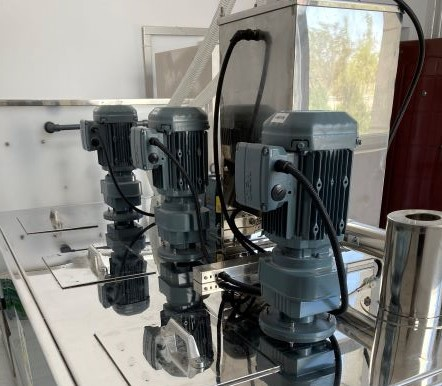
\includegraphics[height=5.5cm]{g15.JPG}};

                    %说明
                    \node at (-5,2) (2) [text_box] {料斗高料位探头};
                    \draw [arrow] (2) -- (0.5,2.2);
                    \draw (0.5,2.2) circle (0.5)[red];
                    \node at (-5,-1) (1) [text_box] {料斗低料位探头};
                    \draw [arrow] (1) -- (0.5,-0.2);
                    \draw (0.5,-0.2) circle (0.5)[red];

                    %辅助线
                    % \draw (-8,-2) [help lines] grid (8,2);
                    % \draw [red] (-8,0) -- (8,0);
                    % \draw [red] (0,-2) -- (0,2);
                \end{tikzpicture}
                \caption{料斗高低料位探头}\label{fig:p12}
            \end{figure}


            \par 料斗高低料位探头
            位置如上图\ref{fig:p12}所示。
            更换
            料斗高低料位探头
            之前,
            应先清理料斗内残留的PAM固体粉料。
        
        \subsubsection{搅拌机及螺旋进料器检修维护}
            检修维护搅拌机及螺旋进料器,
            特别是从装置上拆卸以及重新安装,
            有可能要打开制备系统的上盖,
            操作上较为复杂,
            建议联系加药系统经销商及售后服务人员处理。

            % 搅拌机及螺旋进料器检修
            % 图片模板
      \begin{figure}[h]
         \centering

         \begin{tikzpicture}
            %定义图像
            \node at (0,0) {\includegraphics[height=10cm]{p11.PNG}};

            %说明
            \def \itemNumber {1};
            \def \centertPoint {0,2.5};
            \node at (1,5) (\itemNumber) [text_box] {搅拌机};
            \draw [arrow] (\itemNumber) -- (\centertPoint);
            \draw (\centertPoint) circle (0.5)[red];

            \def \itemNumber {2};
            \def \centertPoint {-0.2, -3.2};
            \node at (-2,-5) (\itemNumber) [text_box] {放空阀};
            \draw [arrow] (\itemNumber) -- (\centertPoint);
            \draw (\centertPoint) circle (0.5)[red];

            \def \itemNumber {3};
            \def \centertPoint {-1.1, -2.7};
            \node at (-4,-4) (\itemNumber) [text_box] {放空阀};
            \draw [arrow] (\itemNumber) -- (\centertPoint);
            \draw (\centertPoint) circle (0.5)[red];

            \def \itemNumber {4};
            \def \centertPoint {-2.2, -2};
            \node at (-6,-3) (\itemNumber) [text_box] {放空阀};
            \draw [arrow] (\itemNumber) -- (\centertPoint);
            \draw (\centertPoint) circle (0.5)[red];

            \def \itemNumber {5};
            \def \centertPoint {0,1};
            \node at (3,4) (\itemNumber) [text_box] {螺旋进料器};
            \draw [arrow] (\itemNumber) -- (\centertPoint);
            \draw (\centertPoint) circle (0.5)[red];

            \def \itemNumber {6};
            \def \centertPoint {1.7,1.6};
            \node at (5,3) (\itemNumber) [text_box] {搅拌机};
            \draw [arrow] (\itemNumber) -- (\centertPoint);
            \draw (\centertPoint) circle (0.5)[red];

			% 辅助线
             \def \xLimit {5};
             \def \yLimit {5};
             %
			% 辅助线
            \draw (-\xLimit,-\yLimit) [help lines] grid (\xLimit,\yLimit);
            \foreach \x in {-\xLimit, ...,\xLimit}{
               \node [red] at (\x, \yLimit) {\x};
               \node [red] at (\x, -\yLimit) {\x};
               \node [red] at (\x, 0) {\x};
            }
            \foreach \y in {-\yLimit, ...,\yLimit}
                  \node [red] at (-\xLimit, \y) {\y};
            \foreach \y in {-\yLimit, ...,\yLimit}
                  \node [red] at (\xLimit, \y) {\y};
            \foreach \y in {-\yLimit, ...,\yLimit}
                  \node [red] at (0, \y) {\y};


         \end{tikzpicture}
         \caption{搅拌机及螺旋进料器检修}\label{fig:p13}
      \end{figure}



            \par 搅拌机及螺旋进料器 的位置,
            如上图\ref{fig:p13}所示。
            拆卸检修 之前,
            应先打开上图\ref{fig:p13}所示排空阀,
            排尽制备装置内液体。

   \subsection{系统恢复运行}
        设备检修完成后,
        请关闭相应工位的检修排液阀,
        打开加药阀,
        打开供药阀,
        将投加系统的阀门都恢复至正常位置。
        \par 然后,
        请参阅第\ref{sec:sg1}章内容于第\pageref{sec:sg1}页,
        做好设备启动前准备,
        使系统处于待命状态,
        随时恢复正常运行。




\end{document}
